% NOTE: RQ2
\subsubsection{Data shape check ($N = 26$)}

\begin{table}
  \centering
  \caption{Assertions used to check the shape of the data.}
  \begin{tabular}{@{}m{0.05\textwidth} m{0.8\textwidth}@{}}
    \toprule
    \emph{\textbf{Key}}&
    \emph{\textbf{Code}}\\
    \midrule

    A5 &
    \lstinline[]$assert y_valid.shape == (1132,)$\\

    A17 &
    \lstinline[]$assert X.shape[1] == 13, 'Did you drop/lose some columns in X? Did you properly load and split the data?'$\\

    A29 &
    \lstinline[]$assert len(test_y_preds) == len(test_y), 'Unexpected number of predictions.'$\\

    A31 &
    \lstinline[]$assert img.shape == (112, 92)$\\

    A76 &
    \lstinline[]$assert len(encoding['token_type_ids']) == max_seq_length$\\

    A84 &
    \lstinline[]$assert red.get_shape().as_list()[1:] == [224, 224, 1]$\\

    A90 &
    \lstinline[]$assert len(X_train) == 2000$\\

    A93 &
    \lstinline[]$assert temp_embed.shape[0] == stride$\\
    \bottomrule
  \end{tabular}
  \label{tab:assert-shape-check}
\end{table}

\subsubsection{Data validation check ($N = 14$)}

\begin{table}
  \centering
  \caption{Assertions used to perform data validation checks.}
  \begin{tabular}{@{}m{0.05\textwidth} m{0.8\textwidth}@{}}
    \toprule
    \emph{\textbf{Key}}&
    \emph{\textbf{Code}}\\
    \midrule

    A41 &
    \lstinline[]$assert np.all(np.unique(X['smoke'].values) == np.array([0, 1]))$\\

    A44 &
    \lstinline[]$assert abs(min(entity_embedding[low:high]) - max(entity_embedding[low:high])) <= 1$\\

    A46 &
    \lstinline[]$assert np.isclose(stdev_norm, 1.0, atol=1e-16)$\\

    A52 &
    \lstinline[]$assert grouped_users['user_id'].nunique() == user_engagement['user_id'].nunique()$\\

    A65 &
    \lstinline[]$assert np.all(y <= nb_classes)$\\

    A73 &
    \lstinline[]$assert df['clf'].value_counts()[1] == len(df[df['quality'] >= 7])$\\
    \bottomrule
  \end{tabular}
  \label{tab:data-validation}
\end{table}

\subsubsection{Model performance check ($N = 11$)}\label{sec:assert-model-perf}

\begin{table}
  \centering
  \caption{Assertions used to check performance of ML models.}
  \begin{tabular}{@{}m{0.05\textwidth} m{0.8\textwidth}@{}}
    \toprule
    \emph{\textbf{Key}}&
    \emph{\textbf{Code}}\\
    \midrule

    A7 &
    \lstinline[]$assert len(neighbours_1) == 20, "Neighbors don't match!"$\\

    A15 &
    \lstinline[]$assert np.allclose(verify('images/camera_1.jpg', 'bertrand', database, FRmodel), (0.54364836, True))$\\

    A19 &
    \lstinline[]$assert np.allclose(linear_model.coef_, [[1.57104472, 0.92521608]]), 'The model parameters you learned seem incorrect!'$\\

    A38 &
    \lstinline[]$assert 0.75 < auc(fpr, tpr) < 0.85$\\

    A58 &
    \lstinline[]$assert np.isclose(accuracy, 0.9666666666666667)$\\
    \bottomrule
  \end{tabular}
  \label{tab:model-perf-explicit}
\end{table}

\subsubsection{Existence check ($N = 8$)}

\begin{table}
  \centering
  \caption{Assertions used to perform existence checks.}
  \begin{tabular}{@{}m{0.05\textwidth} m{0.8\textwidth}@{}}
    \toprule
    \emph{\textbf{Key}}&
    \emph{\textbf{Code}}\\
    \midrule

    A23 &
    \lstinline[]$assert np.all(orders.groupby('user_id') .days_since_prior_order.tail(1).notnull())$\\

    A42 &
    \lstinline[]$assert not lab_s.isnull().values.any()$\\

    A43 &
    \lstinline[]$assert len(data) != 0, 'cannot divide by zero'$\\

    A50 &
    \lstinline[]$assert not np.any(np.isnan(X))$\\

    A51 &
    \lstinline[]$assert data.target.notnull().all()$\\

    A63 &
    \lstinline[]$assert X.isnull().sum().sum() == 0$\\

    A79 &
    \lstinline[]$assert not processed_data_df.isna().any().any()$\\

    A86 &
    \lstinline[]$assert p0 in poi_info.index$\\
    \bottomrule
  \end{tabular}
  \label{tab:existence-check}
\end{table}

\subsubsection{Resource check ($N = 7$)}

\begin{table}
  \centering
  \begin{tabular}{@{}m{0.05\textwidth} m{0.8\textwidth}@{}}
    \toprule
    \emph{\textbf{Key}}&
    \emph{\textbf{Code}}\\
    \midrule

    A10 &
    \lstinline[]$assert le_path.is_file(), f"Label encoder file not found at {le_path}. Make sure 'label_encoder.pkl' exists in the lightning_logs directory."$\\

    A14 &
    \lstinline[]$assert self.model is not None, 'Model is not loaded, load it by calling .load_model()'$\\

    A18&
    \lstinline[]$assert pd.__version__.rpartition('.')[0] == '1.0', f"Unexpected pandas version: expected 1.0, got {pd.__version__.rpartition('.')[0]}"$\\

    A37 &
    \lstinline[]$assert svm.fit_status_ == 0, 'Forgot to train the SVM!'$\\

    A60 &
    \lstinline[]$assert f2.gca().has_data()$\\

    A67&
    \lstinline[]$assert pm.__version__ == '3.9.2'$\\

    A74 &
    \lstinline[]$assert os.path.exists(image_dir)$\\
    \bottomrule
  \end{tabular}
  \caption{Assertions used to validate availability of resources.}
  \label{tab:assert-resource-check}
\end{table}

\subsubsection{Type check ($N = 5$)}

\begin{table}
  \centering
  \caption{Assertions used to check the data type of features in the dataset.}
  \begin{tabular}{@{}m{0.05\textwidth} m{0.8\textwidth}@{}}
    \toprule
    \emph{\textbf{Key}}&
    \emph{\textbf{Code}}\\
    \midrule

    A2 &
    \lstinline[]$assert isinstance(X_trn, torch.FloatTensor), 'Features should be float32!'$\\

    A35 &
    \lstinline[]$assert isinstance(column_transformer, ColumnTransformer), "Input isn't a ColumnTransformer"$\\

    A40 &
    \lstinline[]$assert isinstance(model_3, sklearn.ensemble.RandomForestClassifier)$\\

    A81 &
    \lstinline[]$assert is_all_ints(filled_df[r]) is True$\\

    A88 &
    \lstinline[]$assert isinstance(betas, np.ndarray)$\\
    \bottomrule
  \end{tabular}
  \label{tab:assert-type-check}
\end{table}

\subsubsection{Mathematical property check ($N = 4$)}

\begin{table}
  \centering
  \caption{Assertions used to validate mathematical properties of neural networks.}
  \begin{tabular}{@{}m{0.05\textwidth} m{0.8\textwidth}@{}}
    \toprule
    \emph{\textbf{Key}}&
    \emph{\textbf{Code}}\\
    \midrule

    A3 &
    \lstinline[]$assert (xH - wH) % self.stride == 0$\\

    A25 &
    \lstinline[]$assert test_output.std() < 0.15, "Don't use batchnorm here"$\\

    A56 &
    \lstinline[]$assert np.allclose(e_v_states[:, -1], np.ones_like(e_v_states[:, -1]))$\\

    A64 &
    \lstinline[]$assert np.allclose(T, T.T)$\\
    \bottomrule
  \end{tabular}
  \label{tab:maths-check}
\end{table}

\subsubsection{Batch size check ($N = 3$)}

\begin{table}
  \centering
  \caption{Assertions used to validate the batch size of input data.}
  \begin{tabular}{@{}m{0.05\textwidth} m{0.8\textwidth}@{}}
    \toprule
    \emph{\textbf{Key}}&
    \emph{\textbf{Code}}\\
    \midrule

    A21 &
    \lstinline[]$assert x.size(0) % batch_size == 0, f'the first dimension of input tensor ({x.size(0)}) should be divisible by batch_size ({batch_size})'$\\

    A28 &
    \lstinline[]$assert image_size % patch_size_small == 0, 'Image dimensions must be divisible by the patch size.'$\\

    A70 &
    \lstinline[]$assert n_img > batch_size$\\
    \bottomrule
  \end{tabular}
  \label{tab:batch-size}
\end{table}

\subsubsection{Network architecture check ($N = 3$)}

\begin{table}
  \centering
  \caption{Assertions used to check the architecture of neural networks.}
  \begin{tabular}{@{}m{0.05\textwidth} m{0.8\textwidth}@{}}
    \toprule
    \emph{\textbf{Key}}&
    \emph{\textbf{Code}}\\
    \midrule

    A11 &
    \lstinline[]$assert self.encoder_conv_01[0].weight.size() == self.vgg16.features[2].weight.size()$\\

    A62 &
    \lstinline[]$assert activations[i + 1].shape[1] == self.encoder_layer_sizes[-1] * 2$\\

    A75 &
    \lstinline[]$assert reg in ['none', 'l2']$\\
    \bottomrule
  \end{tabular}
  \label{tab:assert-network-architecture}
\end{table}

\subsubsection{Data leakage check ($N = 1$)}

\begin{table}
  \centering
  \caption{Assert used to prevent data leakage.}
  \begin{tabular}{@{}m{0.05\textwidth} m{0.8\textwidth}@{}}
    \toprule
    \emph{\textbf{Key}}&
    \emph{\textbf{Code}}\\
    \midrule

    A33&
    \lstinline[]$assert len(set( tr_df.PetID.unique()).intersection(valid_df.PetID.unique())) == 0$\\
    \bottomrule
  \end{tabular}
  \label{tab:data-leakage}
\end{table}

% NOTE: RQ3
\subsubsection{Model performance check ($N = 33$)}

\begin{table}
  \centering
  \caption{Various cell outputs used to check the performance of an ML model after training.}
  \begin{tabular}{@{}m{0.05\textwidth} m{0.4\textwidth} m{0.4\textwidth}@{}}
    \toprule
    \emph{\textbf{Key}}&
    \emph{\textbf{Code}}&
    \emph{\textbf{Visual Output}}\\
    \midrule

    P3&
    \lstinline[]$print('The mean accuracy with 10 fold cross validation is: %s ' % round(scores * 100, 2), '%')$&
    \\

    P6&
    \lstinline[]$print('RMSE:', np.sqrt(metrics.mean_squared_error(y_test, pred)))$&
    \\

    P18&
    \lstinline[]$print('The Accuracy is:', accuracy_score(y_test, y_pred))$&
    \\

    P50&
    \lstinline[]$print('Classification Report: SVM (validation data)')$&
    \\

    P54&
    \lstinline[]$print('Intercept value:', lm.intercept_)$&
    \\

    O3&
    \lstinline[]$skplt.metrics. plot_confusion_matrix(Y_val, Vote.predict(X_val), normalize=True, figsize=(10, 10))$&
    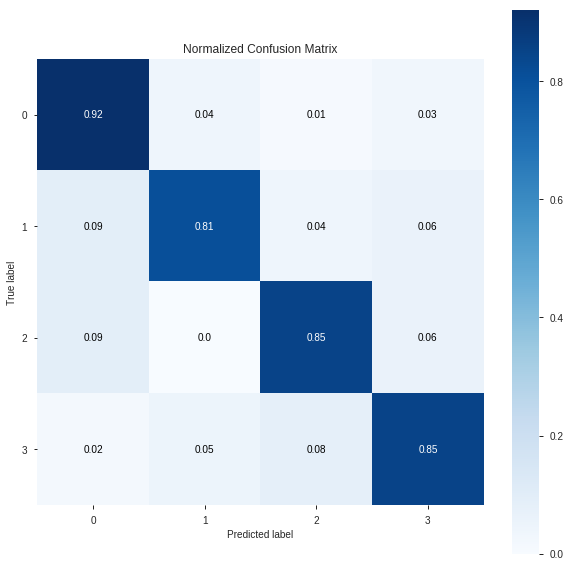
\includegraphics[width=\linewidth]{model-perf-confusion-matrix.png}\\

    O52&
    \lstinline[]$spot_check_recs(classifier, 910)$&
    \\
    \bottomrule
  \end{tabular}
  \label{tab:model-perf}
\end{table}

\subsubsection{Data distribution check ($N = 7$)}~\label{sec:data-distribution-output}

\begin{table}
  \centering
  \caption{Examples of cell outputs used to verify distribution of data.}
  \begin{tabular}{@{}m{0.05\textwidth} m{0.4\textwidth} m{0.4\textwidth}@{}}
    \toprule
    \emph{\textbf{Key}}&
    \emph{\textbf{Code}}&
    \emph{\textbf{Visual Output}}\\
    \midrule

    O2&
    \lstinline[]$_ = sns.catplot(x='category_id', y='likes', data=train, height=5, aspect=1.5)$&
    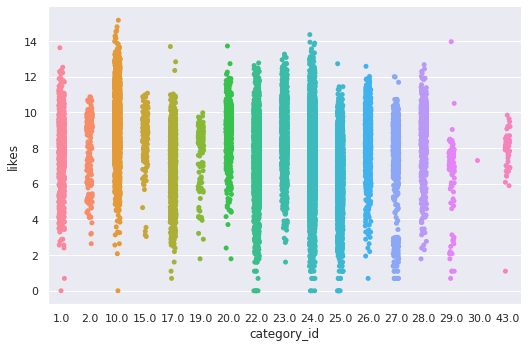
\includegraphics[width=\linewidth]{distribution-check-catplot.png}\\

    O9&
    \lstinline[]$sns.kdeplot(data=data.loc[ data['Survived'] == 0].Age, label='Died', shade=True)$&
    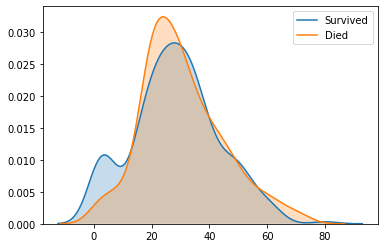
\includegraphics[width=\linewidth]{distribution-check-kdeplot.png}\\

    O14&
    \lstinline[]$pd.pivot_table(train, index='Survived', values=['Age', 'SibSp', 'Parch', 'Fare'])$&
    \\

    O25&
    \lstinline[]$sns.countplot(house_pred['OverallQual'])$&
    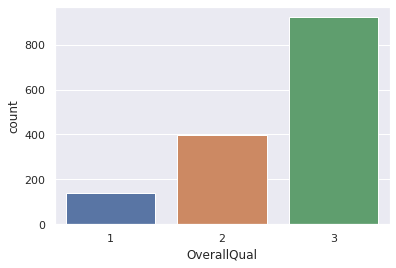
\includegraphics[width=\linewidth]{o25.png}\\

    O48&
    \lstinline[]$x_train.describe()$&
    \\

    \bottomrule
  \end{tabular}
  \label{tab:distribution-check}
\end{table}

\subsubsection{Resource check ($N = 7$)}\label{sec:implicit-resource-check}

\begin{table}
  \centering
  \caption{Examples of cell outputs used to verify if different types of resources are available on the system where the notebook is being executed.}
  \begin{tabular}{@{}m{0.05\textwidth} m{0.8\textwidth}@{}}
    \toprule
    \emph{\textbf{Key}}&
    \emph{\textbf{Code}}\\
    \midrule

    P68&
    \lstinline[]$print('GPU is available')$\\

    P71&
    \lstinline[]$print('Hub version: ', hub.__version__)$\\

    P82&
    \lstinline[]$print('Running on TPU ', tpu.master())$\\

    P86&
    \lstinline[]$print('Cuda is available')$\\

    P107&
    \lstinline[]$print('Model loaded')$\\

    O64&
    \lstinline[]$full_table.head(-5)$\\

    O66&
    \lstinline[]$prostate_cancer_df.shape$\\
    \bottomrule
  \end{tabular}
  \label{tab:resource-check}
\end{table}

\subsubsection{Spot check ($N = 5$)}

\begin{table}
  \centering
  \caption{Example of outputs used to perform spot checks.}
  \begin{tabular}{@{}m{0.05\textwidth} m{0.8\textwidth}@{}}
    \toprule
    \emph{\textbf{Key}}&
    \emph{\textbf{Code}}\\
    \midrule

    O60 &
    \lstinline[]$X_pca.head()$\\

    P64 &
    \lstinline[]$print(np.max(cur[:, :, 1]))$\\

    P114 &
    \lstinline[]$print(onehot_encoded)$\\
    \bottomrule
  \end{tabular}
  \label{tab:spot-check}
\end{table}

\subsubsection{Model training check ($N = 4$)}

\begin{table}
  \centering
  \caption{Example of outputs used to monitor model training.}
  \begin{tabular}{@{}m{0.05\textwidth} m{0.8\textwidth}@{}}
    \toprule
    \emph{\textbf{Key}}&
    \emph{\textbf{Code}}\\
    \midrule

    O8 &
    \lstinline[]$autoencoder.fit(x=X_train, y=X_train, epochs=15, validation_data=[X_test, X_test], callbacks=[keras_utils.TqdmProgressCallback()], verbose=0)$\\

    O31 &
    \lstinline[]$adaBoost.fit(X_train, y_train)$\\

    O42&
    \lstinline[]$m_r.best_params_$\\
    \bottomrule
  \end{tabular}
  \label{tab:model-training}
\end{table}

\subsubsection{Missing value check ($N = 3$)}

\begin{table}
  \centering
  \caption{Examples of cell outputs used to check for missing data.}
  \begin{tabular}{@{}m{0.05\textwidth} m{0.4\textwidth} m{0.4\textwidth}@{}}
    \toprule
    \emph{\textbf{Key}}&
    \emph{\textbf{Code}}&
    \emph{\textbf{Visual Output}}\\
    \midrule

    P74&
    \lstinline[]$print(train_df.isnull().sum())$\\

    L12&
    \lstinline[]$sns.heatmap(test_df.isnull(), yticklabels=False, cbar=False, cmap='viridis')$&
    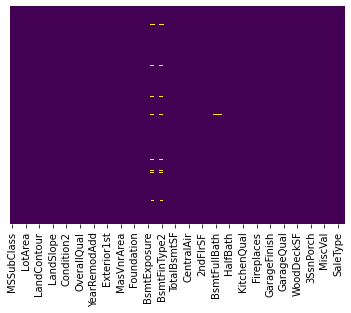
\includegraphics[width=\linewidth]{missing-value-check.png}\\

    L36&
    \lstinline[]$test.isna().sum().unique()$\\
    \bottomrule
  \end{tabular}
  \label{tab:missing-value}
\end{table}

\subsubsection{Shape check ($N = 3$)}

\begin{table}
  \centering
  \caption{Example of outputs used to check the shape of the data.}
  \begin{tabular}{@{}m{0.05\textwidth} m{0.8\textwidth}@{}}
    \toprule
    \emph{\textbf{Key}} & \emph{\textbf{Code}}\\
    \midrule
    P4 &
    \lstinline[]$print('no.of examples in test data : ', len(test_data))$\\

    P32 &
    \lstinline[]$print('Training set shape : ', x_train.shape)$\\

    P117&
    \lstinline[]$print('Y_train.shape: ', Y_train.shape)$\\
    \bottomrule
  \end{tabular}
  \label{tab:shape-check}
\end{table}

\subsubsection{Data relationship check ($N = 2$)}~\label{sec:linear-relation-output}

\begin{table}
  \centering
  \caption{Cell outputs used to verify linear relationship between features in the data.}
  \begin{tabular}{@{}m{0.05\textwidth} m{0.4\textwidth} m{0.4\textwidth}@{}}
    \toprule
    \emph{\textbf{Key}}&
    \emph{\textbf{Code}}&
    \emph{\textbf{Output}}\\
    \midrule

    O6&
    \lstinline[]$b = sns.relplot(x='SIZE', y='Cash', hue='CLARITY', alpha=0.9, palette='muted', height=8, data=raw_data)$&
    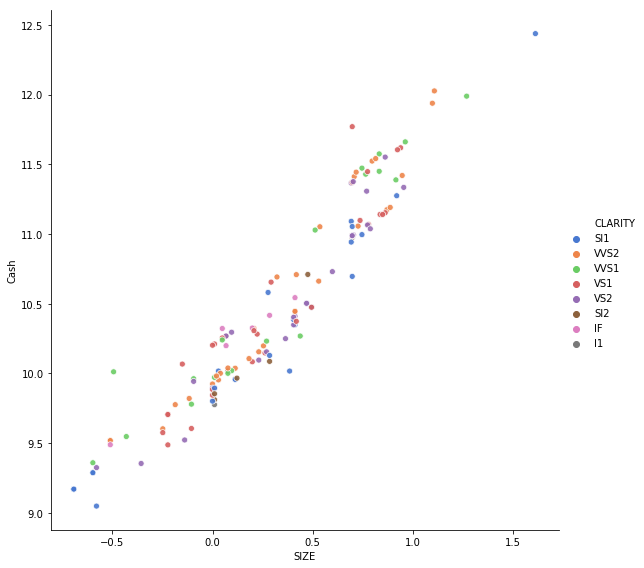
\includegraphics[width=\linewidth]{linear-relation-check-lineplot.png}\\

    O10&
    \lstinline[]$sns.regplot(x='X4 number of convenience stores', y='Y house price of unit area', data=data)$&
    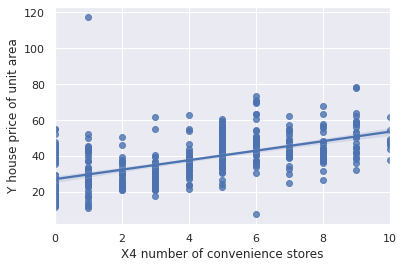
\includegraphics[width=\linewidth]{linear-relation-check-regplot.png}\\
    \bottomrule
  \end{tabular}
\label{tab:linear-relation-check}
\end{table}

\subsubsection{Type check ($N = 2$)}

\begin{table}
  \centering
  \caption{Outputs used to check the data type of features in the data.}
  \begin{tabular}{@{}m{0.05\textwidth} m{0.8\textwidth}@{}}
    \toprule
    \emph{\textbf{Key}} &
    \emph{\textbf{Code}}\\

    P43&
    \lstinline[]$print('data type:', images.dtype)$\\

    O71&
    \lstinline[]$type(Y)$\\
    \bottomrule
  \end{tabular}
  \label{tab:type-check}
\end{table}

\subsubsection{Execution time check ($N = 1$)}

\begin{table}
  \centering
  \caption{Print statement used to check the total execution time of training and cross-validating an ML model.}
  \begin{tabular}{@{}m{0.05\textwidth} m{0.8\textwidth}@{}}
    \toprule
    \emph{\textbf{Key}}&
    \emph{\textbf{Code}}\\
    \midrule

    P66&
    \lstinline[]$print('Total Run Time:')$\\
    \bottomrule
  \end{tabular}
  \label{tab:exec-time}
\end{table}

\subsubsection{Network architecture check ($N = 1$)}

\begin{table}
  \centering
  \caption{Print the architecture of a neural network.}
  \begin{tabular}{@{}m{0.05\textwidth} m{0.8\textwidth}@{}}
    \toprule
    \emph{\textbf{Key}}&
    \emph{\textbf{Code}}\\
    \midrule
    P92&
    \lstinline[]$print(MyNetwork)$\\
    \bottomrule
  \end{tabular}
  \label{tab:network-architecture}
\end{table}
